\documentclass[../SimBALink.tex]{subfiles}
\begin{document}

\section{Block diagram}
	\begin{figure}[h]
			\centering
			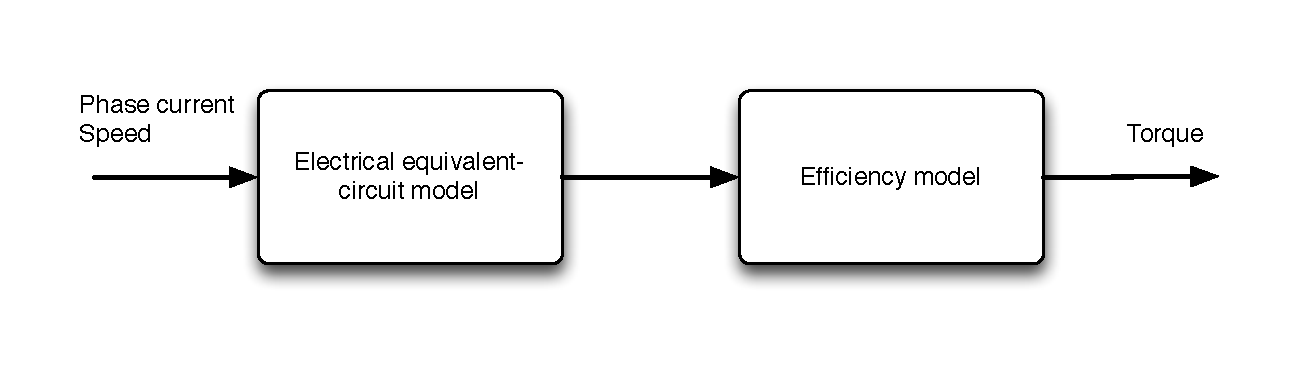
\includegraphics[width=\linewidth]{../Model/Powertrain/Motor/Documentation/Figures/Motor_block_diagram}
			\caption{Motor model block diagram.}
	\end{figure}
	\FloatBarrier

\section{Inputs and outputs}
	\subsection{Inputs}
	\begin{tabular}{ r | c | l | l }
		Signal						&	Symbol				&	MATLAB variable	&	Unit						\\\hline	
		Stator current					&	$I_s$				&	\texttt{Is}			&	rms amps					\\
		Stator current (quadrature axis)	&	$I_q$				&	\texttt{Is.Iq}		&	rms amps			\\
		Stator current (direct axis)		&	$I_d$				&	\texttt{Is.Id}		&	rms amps			\\
		Motor speed					&	$\omega$			&	\texttt{omega}		&	rad/sec
	\end{tabular}
	
	\subsection{Outputs}
		\begin{tabular}{ r | c | l | l }
			Signal						&	Symbol				&	MATLAB variable	&	Unit						\\\hline	
			Motor torque					&	$\tau$				&	\texttt{tau}		&		N m				\\
		\end{tabular}
	
\section{Background, rationale, modeling strategy}
	The motor model has two main components. The torque-generation component is based on an electrical equivalent-circuit model and a 2D efficiency map derived from motor-specific testing. There is also a simple thermal model based on a constant thermal resistance.
	
	\subsection{Torque model}
		The motor's electrical behavior can be represented using two equivalent circuits using the Park transformation \cite{Park1929}. The result of the transformation for a 3-phase permanent-magnet synchronous motor (PMSM) is the \textit{dq} motor model. Figure \ref{fig:Motor_equivalent_circuit} shows the constant-parameter \textit{dq} equivalent circuits.
		
		\begin{figure}[h]
			\centering
			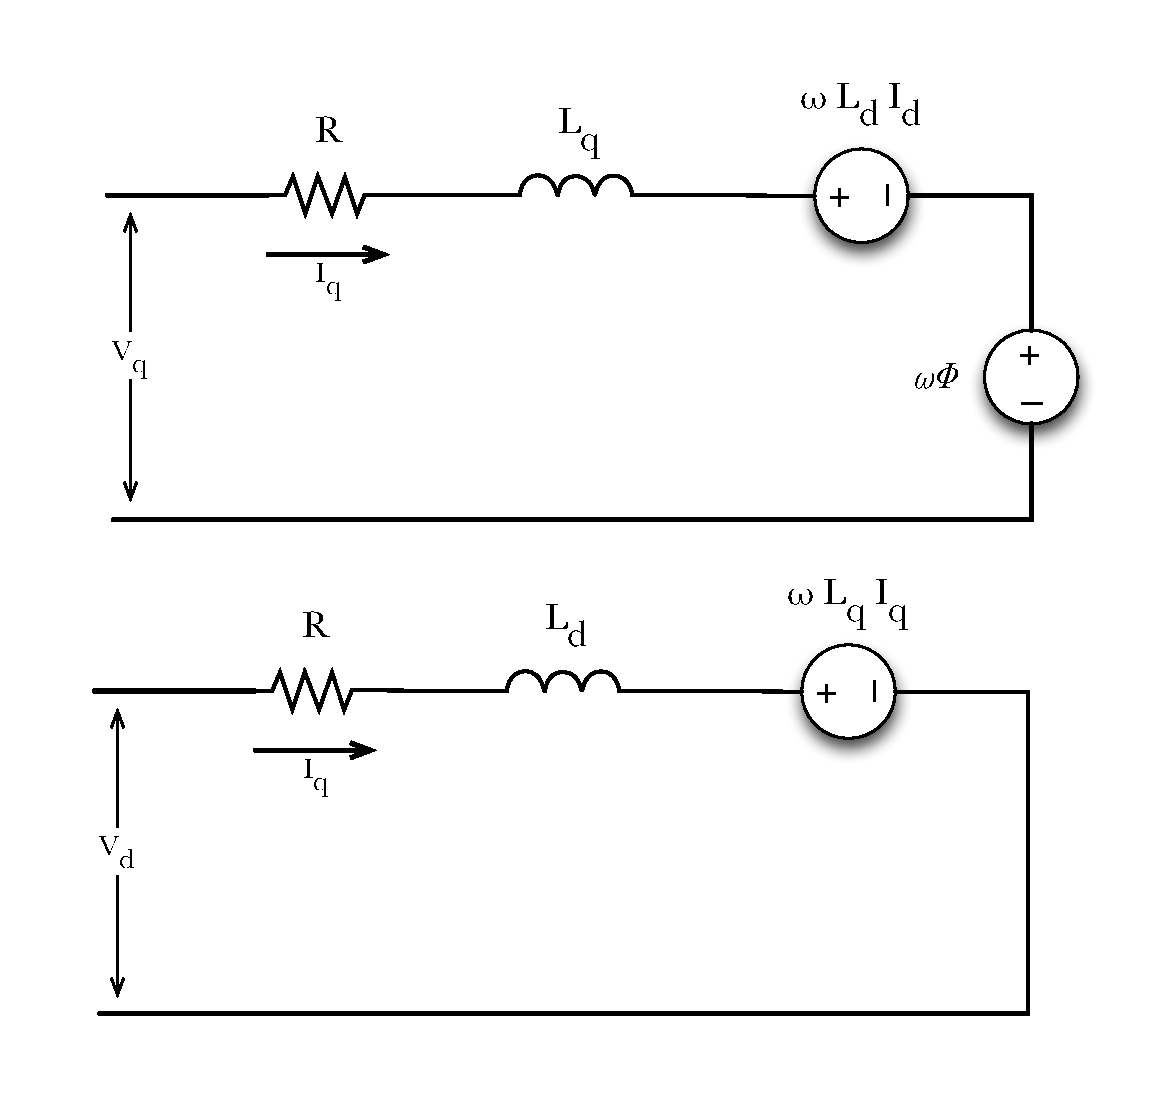
\includegraphics[width=\linewidth]{../Model/Powertrain/Motor/Documentation/Figures/Motor_equivalent_circuit}
			\caption{Motor model - \textit{dq} equivalent circuits.}
			\label{fig:Motor_equivalent_circuit}
		\end{figure}
		\FloatBarrier
		
		The motor parameters are assumed to be constant with respect to stator currents and temperatures.
		
		By the equivalent circuits in Figure \ref{fig:Motor_equivalent_circuit}, the stator voltages $V_d$ and $V_q$ can be found:
		
		\begin{gather}
			V_d		= R i_d + L_d \frac{ d i_d }{ d t } + \omega L_q i_q				\label{eqn:Vd_with_Vl}\\
			V_q		= R i_q + L_d \frac{ d i_q }{ d t } + \omega L_d i_d	- \omega \phi	\label{eqn:Vq_with_Vl}
		\end{gather}
		
		Calibrating the above model using experimental data could be difficult because of the $\frac{d i}{d t}$ terms. After evaluating typical values of $\frac{d i_q}{d t}$ recorded in previous testing, the maximum observed value (about -3070 A/sec) was small enough that the inductance term $L \frac{d i}{d t}$ could be neglected without introducing significant error. With this modification, \ref{eqn:Vd_with_Vl} and \ref{eqn:Vq_with_Vl} become
		
		\begin{gather}
			V_d		= R i_d + \omega L_q i_q				\label{eqn:Vd_without_Vl}\\
			V_q		= R i_q + \omega L_d i_d - \omega \phi		\label{eqn:Vq_without_Vl}
		\end{gather}
		
		It is assumed that the power inverter has perfect control over the $d$- and $q$-axis currents $I_d$ and $I_q$. With the known stator current $I_s = \sqrt{I_d^2 + I_q^2}$, the input power can be found:
		
		\begin{equation}
			P_e = I_s \times V_s
		\end{equation}
		
		Then the motor "electrical torque" can be found:
		
		\begin{equation}
			\tau_e = \frac{P_e}{\omega}
		\end{equation}
		
		The motor output torque is the product of $\tau_e$ and the motor efficiency:
		
		\begin{equation}
			\tau	=	\eta(\tau_e, \omega) \times \tau_e
		\end{equation}

\section{Parameters}
	
	\renewcommand{\arraystretch}{1.5}
	\begin{tabular}{ p{5cm} | c | l | l }
		Parameter					&	Symbol				&	MATLAB variable	&	Unit						\\\hline	
		Q-axis inductance				&	$L_q$				&	\texttt{Lq}			&	H			\\
		D-axis inductance				&	$L_d$				&	\texttt{Ld}			&	H			\\
		Equivalent-circuit series resistance	&	$R$					&	\texttt{R}			&	ohm			\\
		Permanent-magnet flux linkage	&	$\phi_m$				&	\texttt{phi}		&	V s $\text{rad}^{-1}$	\\
		Motor efficiency				&	$\eta$				&	\texttt{eta}		&				\\
		Motor efficiency lookup: stator current breakpoints	&			&	\texttt{eta.Is}		&	rms amps ($I_s$)	\\
		Motor efficiency lookup: motor speed breakpoints	&			&	\texttt{eta.omega}	& 	rad/sec		\\
		Motor efficiency data			&						&	\texttt{eta.eta\_m}	&	
	\end{tabular}


\section{Assumptions}
	The motor electrical model is significantly simplified.
	\begin{itemize}
		\item 
			The model assumes that the motor magnetization is linear (i.e., the motor never saturates).
		\item
			The model assumes that the motor inductances $L_d$ and $L_q$ are constant. In fact, \todo{details about behavior of Lq with Id}
		\item
			The motor efficiency model assumes that motor efficiency $\eta$ depends only on motor speed and electrical torque.
	\end{itemize}

\bibliographystyle{plain}
\bibliography{bib/SimBALink}

\end{document}